\documentclass[12pt, oneside, a4paper]{report}

\usepackage[left=3.5cm, top=2.5cm, bottom=2.5cm, right=2.5cm]{geometry}

\usepackage[utf8]{inputenc}
\usepackage[T1]{polski}
\usepackage[polish]{babel}
\usepackage{indentfirst}
\usepackage{graphicx}
\usepackage{mathtools}
\usepackage{natbib}
\setcitestyle{super,open={[},close={]}}

\begin{document}  
\thispagestyle{empty}
\begin{titlepage}
    \begin{center}

           \Large
	\textbf{Uniwersytet Jagielloński w Krakowie}\vspace{0.2cm}\\ Wydział Fizyki, Astronomii i Informatyki Stosowanej
               \vspace*{1cm}
               
         \vspace{3cm}
         \Large
          \textbf{Paweł Sławomir Mstowski}\\\vspace{0.5cm}
         \normalsize Nr albumu: 1148921\\
             \vspace{2cm}
        \Huge
        \textbf{Nauczanie sieci neuronowych za pomocą algorytmu genetycznego na przykładzie samouczącego się bota do gry zręcznościowej.}
      
        \vspace{1.5cm}
        \normalsize
        Praca magisterska\\
        na kierunku Informatyka Stosowana\\ \vspace{0.15cm}
        
        \vfill
        \vspace{2cm}
       \begin{minipage}{1\textwidth}
\begin{flushright}
Praca wykonana pod kierunkiem\\
prof. dr hab. Piotra Białasa\\
Zakład Technologii Gier
\end{flushright}
\end{minipage}
        
        \vspace{2cm}
        \begin{center}
      Kraków 2019
        \end{center}
    \end{center}
\end{titlepage}

\newpage 
 \thispagestyle{empty}
\vspace{2.5cm}
\begin{flushleft}
\large \textbf{Oświadczenie autora pracy}\vspace{0.6cm}\\
\end{flushleft}

\noindent Świadom odpowiedzialności prawnej oświadczam, że niniejsza praca dyplomowa została napisana przeze mnie samodzielnie i nie zawiera treści uzyskanych w sposób niezgodny z obowiązującymi przepisami.\\

\noindent Oświadczam również, że przedstawiona praca nie była wcześniej przedmiotem procedur związanych z uzyskaniem tytułu zawodowego w wyższej uczelni.
\vspace{2cm}
\begin{center}
\begin{tabular}{lr}
................................~~~~~~~~~~~~~~~~~~~~~~~~~~~~~~~~~~~~~~&
.......................................... \\
{~~~~Kraków, dnia} & {Podpis autora pracy~~~~}
\end{tabular}
\end{center}
\vspace{5cm}
\begin{flushleft}
\large \textbf{Oświadczenie kierującego pracą}
\end{flushleft}

\noindent Potwierdzam, że niniejsza praca została przygotowana pod moim kierunkiem i~kwalifikuje się do przedstawienia jej w postępowaniu o nadanie tytułu zawodowego.
\vspace{2cm}
\begin{center}
\begin{tabular}{lr}
................................~~~~~~~~~~~~~~~~~~~~~~~~~~~~~~~~~~~~~~&
............................................ \\
{~~~~Kraków, dnia} & {Podpis kierującego pracą~~}
\end{tabular}
\end{center}
\vfill

%%%%%%%%%%%%%%%%%%%%%%%%%%%%%%%%%%%%%%%%%%%%%%%%%%%%%%%%%%%%%%%%%%%%%%%%%%%%%%%%%%%%%

\tableofcontents

%%%%%%%%%%%%%%%%%%%%%%%%%%%%%%%%%%%%%%%%%%%%%%%%%%%%%%%%%%%%%%%%%%%%%%%%%%%%%%%%%%%%%

\chapter{Wstęp}

(napiszę po wnioskach, będzie to krótkie streszczenie tego co przedstawia praca, jej struktury oraz postawienie tezy)

%%%%%%%%%%%%%%%%%%%%%%%%%%%%%%%%%%%%%%%%%%%%%%%%%%%%%%%%%%%%%%%%%%%%%%%%%%%%%%%%%%%%%

\chapter{Sieci neuronowe}

W rozdziale tym postaram się przybliżyć zagadnienie sztucznych sieci neuronowych. Zacznę od krótkiej historii powstania tej koncepcji oraz idei przyświecającej jej twórcom. Przedstawię budowę elementarnego fragmentu budującego takie sieci czyli sztucznego neuronu i wyjaśnię jego wewnętrzny sposób działania. Potem przejdę do definiowania czym jest sztuczna sieć neuronowa, jakie cechy opisują jej strukturę oraz wymienię jej różne typy. Po naszkicowaniu teorii ich działania przejdę do przedstawienia aktualnych dziedzin zastosowania tych technik na następnie zobrazuję metody nauczania tychże sieci na potrzeby rozwiązywania zadanych problemów.

\section{Czym są sieci neuronowe?}

Sieci neuronowe są to systemy przetwarzania informacji wzorowane na procesach i strukturach obserwowanych w ludzkim mózgu. Pierwszą sztuczną siecią neuronową był perceprton progowy, który został wymyślony w roku 1943 przez Warrena Sturgisa McCullocha i Waltera Pittsa. Wymyślona wtedy koncepcja jest nadal bardzo aktualna i wykorzystywana do dziś. Teraźniejszy poziom zaawansowania komputerów i ich moc obliczeniowa wywołały swego rodzaju renesans badań nad sieciami neuronowymi.

Tak samo jak nasz mózg składa się z setek miliardów komórek neuronowych tak sztuczne sieci neuronowe są tworzone przez setki lub tysiące sztucznych neuronów, które są najmniejszymi elementami przetwarzającymi informację. Są one prymitywną interpretacją sposobu działania prawdziwych, biologicznych neuronów i składają się z wielu wejść oraz jednego wyjścia. Budowa takiego pojedynczego elementu sieci przedstawiona jest poniżej (Rysunek \ref{fig: 2.1}).

\begin{figure}[h]
	\centering
	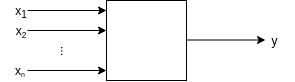
\includegraphics[width=7cm]{fig211.png}
	\caption{Schemat budowy sztucznego neuronu}
	\label{fig: 2.1}
\end{figure}

Każde wejście sztucznego neuronu posiada też swoją wagę, która jest potem używana do obliczenia jego wyjścia. W takim wypadku funkcję każdego pojedynczego elementu sieci możemy zapisać jako (Równanie \ref{eq: 2.1})

\begin{equation}\label{eq: 2.1}
y = \sum^{n}_{i=1} x_{i}w_{i}
\end{equation}

Dodatkowo każdy neuron posiada swoją wartość przesunięcia (ang. \textit{bias}) sygnału. Funkcja wyjścia zaprezentowana powyżej z uwzględnieniem tej wartości będzie wyglądać (Równanie \ref{eq: 2.2}):

\begin{equation}\label{eq: 2.2}
  y = \sum^{n}_{i=1} x_{i}w_{i} + b
\end{equation}

Topologia połączeń oraz ich parametry stanowią program działania sieci \citep{tadeusiewicz1993sieci}. Sygnały wejściowe są przepuszczane przez chmurę połączonych ze sobą neuronów, które następnie przeliczają te sygnały i przekazują swoje rozwiązania dalej w głąb sieci. Tak przetworzone dane dają w wyniku pewną ilość sygnałów wyjściowych z sieci które razem są rozwiązaniem problemu, do którego została wyuczona.

Możemy wyodrębnić kilka podstawowych rodzajów sieci neuronowych na podstawie ich topologii takie jak sieci jedno warstwowe, wielowarstwowe, jednokierunkowe czy rekurencyjne. Każda z tych wariacji jest skuteczna w rozwiązywaniu innych problemów. Dla przykładu sieci jednowarstwowe, które w praktyce składają się z dwóch warstw (warstwa wejściowa nie przetwarza a jedynie przekazuje dane wejściowe do sieci), nadają się do klasyfikowania informacji, które jesteśmy w stanie rozdzielić liniowo. Sieci wielowarstwowe różnią się od jednowarstwowych jedynie dodatkowymi warstwami ukrytymi. W klasycznych sieciach neuronowych połączenia pomiędzy neuronami istnieją jedynie między warstwami. Obraz poniżej prezentuje przykładową wielowarstwową sztuczną sieć neuronową (Rysunek \ref{fig: 2.2})

\begin{figure}[h]
	\centering
	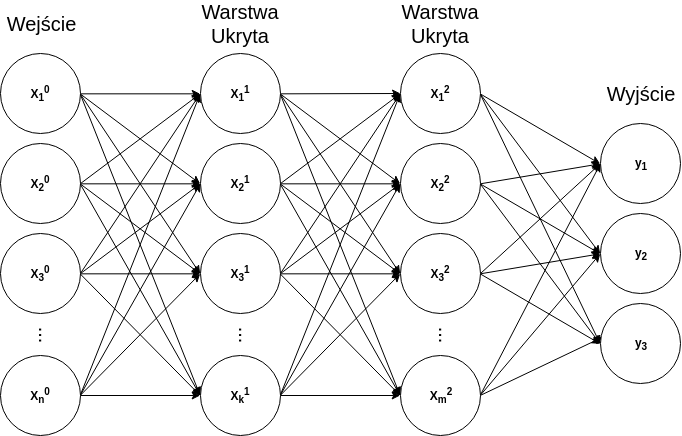
\includegraphics[width=12cm]{fig212.png}
	\caption{Schemat wielowarstwowej sieci neuronowej}
	\label{fig: 2.2}
\end{figure}

Aby jednoznacznie określić konkretną sztuczną sieć neuronową możemy się posłużyć uproszczonym modelem opisanym przez trzy podstawowe cechy takiej sieci. Tymi cechami są architektura, proces uczenia i funkcja aktywacji. Architektura opisuje dokładnie topologię sieci, w tym jej rodzaj oraz liczby warstw i neuronów w każdej warstwie. Uczenie jest opisem procesu zastosowanego do rozwinięcia parametrów sieci. Określa ono poszczególne techniki użyte do tego celu jak na przykład uczenie przez wzmacnianie czy uczenie ze zbioru reguł. Definiuje też zakresy i wartości wag połączeń między neuronami. Ostatnia cecha czyli funkcja aktywacji opisuje sposób wewnętrznego działania neuronu, czyli kiedy będzie on aktywny oraz jakie dane przekaże dalej w głąb sieci.

Istnieje wiele powszechnie używanych funkcji aktywacji neuronów. Najprostszym jej przykładem jest funkcja tożsamości, która przekazuje bezpośrednio na wyjście wartość aktywacji neuronu i jest wyrażana wzorem (Równanie \ref{eq: 2.3})

\begin{equation}\label{eq: 2.3}
  f(a) = a
\end{equation}

Innym przykładem jest funkcja nazywana \textbf{ReLU}(\textit{Rectified Linear Unit}) i najbardziej ze wszystkich odzwierciedla sposób aktywacji neuronu biologicznego (Równanie \ref{eq: 2.4}).

\begin{equation}\label{eq: 2.4}
    f(a) =
    \begin{cases*}
      a & if a $\geq$ 0 \\
      0 & if a < 0
    \end{cases*}
\end{equation}

Powyższa funkcja jest połączeniem funkcji tożsamości oraz funkcji progowej, która na wyjściu zwraca tylko informację czy została aktywowana i opisuje ją wzór (Równanie \ref{eq: 2.5})

\begin{equation}\label{eq: 2.5}
  f(a) =
  \begin{cases*}
    1 & if a $\geq$ 0 \\
    0 & if a < 0
  \end{cases*}
\end{equation}

Istnieją również bardziej zaawansowane funkcje aktywacji. Jedną z najczęściej używanych jest funkcja logistyczna (Równanie \ref{eq: 2.6}), która zwraca wartość mięczy 0 a 1 i jej wynik jest określany jako prawdopodobieństwo aktywacji neuronu.

\begin{equation}\label{eq: 2.6}
  f(a) = \frac{1}{1 + exp(-a)}
\end{equation}

\section{Zastosowania sieci neuronowych}

Bazując na wcześniej podanych informacjach można powiedzieć, że sztuczne sieci neuronowe pomimo swojej genezy nie są idealnym odzwierciedleniem sposobu działania swojego pierwowzoru, czyli ludzkiego mózgu. Przez swoje ograniczenia ich zdolności do rozwiązywania problemów są ograniczane. Każda sieć neuronowa jest projektowana i uczona do rozwiązywania konkretnego problemu i nie radzi sobie z danymi związanymi z innymi zagadnieniami niż jej specjalizacja. Z podstaw działania sztucznego neuronu można wywnioskować, że ma on zdolność do rozpoznawania wzorców na podstawie porównania otrzymanych sygnałów do swojego wektora wag. Z tego wynika, że sztuczne neurony połączone w skomplikowaną sieć są idealne do takich zadań na dużo większą skalę. Taki sposób działania pozwala na wykorzystanie tych mechanizmów w wielu branżach.

Aktualnie sieci neuronowe są używane do przetwarzania danych w bardzo dużym spektrum dziedzin. Ich zastosowania można znaleźć przedmiotach codziennego użytku takich jak smartfony, na przykład do rozpoznawania mowy i implementacji interfejsów głosowych, jak też w bardzo profesjonalnych sprzętach i systemach. Na podstawie wcześniej dostarczonych danych jesteśmy w stanie nauczyć sieci neuronowe przewidywać pewne zdarzenia na podstawie aktualnych danych. Wiele firm w dzisiejszych czasach tworzy systemy, które na podstawie parametrów technicznych urządzeń w zakładach są wstanie podać bardzo dokładne prawdopodobieństwo awarii danego sprzętu. Sztuczne sieci neuronowe zostały wykorzystane przez różnych badaczy do modelowania i prognozowania w dziedzinie systemów inżynierii energetycznej \citep{kalogirou2000applications}. Współczesna medycyna generuje zawrotne ilości danych korzystając z zaawansowanych czujników monitorujących. Potencjalne zastosowania takich danych obejmują dokładne klasyfikowanie diagnoz, przewidywanie przyszłych chorób i śmiertelności \citep{lipton2015learning}.

Zastosowanie sieci neuronowych w dzisiejszych czasach jest bardzo dobrze widoczne w dziedzinie rozpoznawania obrazów. Wydajność i dokładność algorytmów tworzonych do tych celów może być w łatwy sposób mierzona poprzez porównanie wyniów ich działania na popularnej bazie ImageNet \citep{image-net} zawierającej szesnaście milionów zdjęć. W czasach małej popularności sieci neuronowych sprawność algorytmów rozpoznawania obrazów rozwijała się bardzo powoli. Jednakże w okresie wzmożonego wprowadzania rozwiązań z tematyki sieci neuronowych do tejże dziedziny możemy zaobserwować znaczny spadek stopy błędu z 40\% w roku 2010 do zaledwie 7\% w roku 2014. Ze względu na sukces głębokich sieci neuronowych wszyscy uczestnicy współzawodnictwa ImageNet w 2013 roku zastosowali jakąś formę głębokiej sieci neuronowej \citep{roelants2017deeplearning}.

Często wyuczone sieci odzwierciedlają swoim działaniem algorytmy, które już zostały wymyślone. Jednakże sposób w jaki to robią może dostarczyć nowych spostrzeżeń dotyczących rozwiązywanego problemu i lepszych implementacji algorytmów \citep{murray1995applications}.


\section{Metody nauczania sieci neuronowych}

Pod pojęciem nauczania sieci neuronowej, zwanego też uczeniem maszynowym, kryją się różne procesy prowadzące do takiej modyfikacji wszystkich wag w sieci aby jak najlepiej rozwiązywała dany problem. Techniki uczenia maszynowego można zgrubnie podzielić na dwie duże klasy: uczenie nadzorowane i nienadzorowane, choć dość często dodawana jest też trzecia klasa - tzw. uczenie przez wzmacnianie \citep{roelants2017deeplearning}. Każda z tych klas wymaga dostarczenia innych danych do poprawnego działania. W niektórych przypadkach musimy dysponować dużą ilością informacji wstępnie sklasyfikowanych, żeby sieć na ich przykładzie mogła się uczyć a w innych potrzebujemy po prostu surowych danych, które taka sieć sklasyfikuje samodzielnie.

Uczenie nadzorowane jest pierwsza wymienioną przeze mnie klasą algorytmów nauczania maszynowego. Zaliczają się do niej algorytmy korzystające z zestawów danych treningowych, które są wstępnie opracowywane i oznaczane oczekiwanymi etykietami (etykietowane) ręcznie przez osoby nadzorujące uczenie sieci. Samo uczenie odbywa się poprzez zmiany w zestawie wag sieci, które dążą zo zminimalizowania wartości funkcji błędu określanej przez różnicę między wyjściem sieci a właśnie oczekiwanymi etykietami. W konsekwencji działania takiego algorytmu otrzymujemy sieć neuronową, której wagi wyznaczają \textit{k-1} hiperpłaszczyzn w \textit{n-wymiarowej} przestrzeni, gdzie \textit{k} jest liczbą oczekiwanych klas a \textit{n} ilością neuronów wejściowych sieci.

Kolejną klasą algorytmów jest uczenie nienadzorowane, które stając po przeciwnej stronie do poprzednio zaprezentowanego uczenia nadzorowanego nie korzysta z wcześniej etykietowanych danych. Najlepszym przykładem działania tych algorytmów jest grupowanie otrzymanych danych poprzez wyszukanie odpowiedniej ilości klas danych tak aby poszczególne elementy tych grup cechowały się jak największym podobieństwie do siebie i jak najmniejszym podobieństwem do elementów innych grup.

Ostatnią zaprezentowaną klasą algorytmów było uczenie przez wzmacnianie. Działa ono podobnie do nienadzorowanego ale wykorzystuje też mechanikę sprzężenia zwrotnego z uczenia nadzorowanego. Algorytmy uczenia się przez wzmacnianie zwykle ponownie wykorzystują stosowane w przeszłości działania prowadzące do uzyskania pomyślnych rezultatów \citep{roelants2017deeplearning}.

(muszę uzupełnić jeszcze ten podrozdział o trochę więcej informacji)

%%%%%%%%%%%%%%%%%%%%%%%%%%%%%%%%%%%%%%%%%%%%%%%%%%%%%%%%%%%%%%%%%%%%%%%%%%%%%%%%%%%%%

\chapter{Algorytmy genetyczne}

Poniższy rozdział jest krótkim wprowadzeniem do tematyki algorytmów genetycznych. Będzie on obejmował wszystkie podstawowe zagadnienia potrzebne do zrozumienia działania tych algorytmów takie jak osobnik, populacja czy genotyp. Przedstawię w nim też ogólny schemat działania oraz po krótce wyjaśnię co dzieje się w poszczególnych jego krokach. Potem przejdę do wyjaśniania zagadnienia kodowania rozwiązań na potrzeby algorytmu genetycznego aby pod koniec opisać niektóre z dziedzin, których owe algorytmy znajdują zastosowanie w dzisiejszych czasach.

\section{Wprowadzenie do algorytmów genetycznych}

Wiele rozwiązań z dziedziny informatyki czerpie garściami z procesów i interakcji możliwych do zaobserwowania w otaczającym nas świecie. Dobrym przykładem takiej tendencji jest choćby obiektowy paradygmat programowania zamykający kod w ramy odzwierciedlające doświadczalny świat rzeczywisty. Również przedstawione wcześniej w tej pracy rozwiązania jak sztuczne sieci neuronowe są mocno inspirowane innymi procesami obserwowanymi w przyrodzie a mianowicie sposobem działania ludzkiego mózgu. 

Tak samo jest też z algorytmem genetycznym. Został on zaprojektowany na postawie ogólnej teorii rozwoju życia sformułowanej przez Karola Darwina a jego autorem jest amerykański naukowiec, profesor psychologii, elektroniki i informatyki John Henry Holland. W uproszczeniu można powiedzieć, że algorytmy genetyczne są procedurami poszukiwania opartymi na mechanizmach doboru naturalnego oraz dziedziczności \citep{goldberg1995algorytmygenetyczne}. Podczas projektowania tych algorytmów Panu Holland'owi oraz jego współpracownikom z Uniwersytetu Michigan przyświecały dwa cele. Jednym z nich było jak najprostsze opisanie obserwowalnych w świecie przyrody mechanizmów adaptacyjnych. Drugim zaś wykorzystanie tych informacji do opracowania oprogramowania rozwiązującego skompilowane problemy z wykorzystaniem tychże właśnie procesów i mechanizmów. Według David'a Goldberg'a cała istota funkcjonowania algorytmów genetycznych rozbija się o zachowanie idealnej równowagi między efektywnością a skutecznością szukanych rozwiązań w danym środowisku, które jest definiowane przez dziedzinę problemu. Ten złoty środek nazywa on odpornością. Jest to cecha, której rozwój do perfekcji opanowały wszelakie systemy biologiczne i dlatego zainspirowała on powstanie takich metod w dziedzinie informatyki.

Algorytmy genetyczne są narzędziem wykazującym się dużą efektywnością w przeszukiwaniu skomplikowanych przestrzeni co w ciągu wielu lat zostało wielokrotnie potwierdzone tak w teorii jak i empirycznie. Bardzo dobrze dają sobie również radę w rozwiązywaniu problemów z dziedziny optymalizacji. Jednocześnie dzięki analogiom ich działania do procesów obserwowalnych w przyrodzie cechują niezwykłą łatwością implementacji. Są wyjątkowo nieskomplikowanym a jednocześnie bardzo potężnym narzędziem w szukaniu rozwiązań problemów \textit{NP-Trudnych}.

Działanie wszystkich algorytmów genetycznych zaczynamy od wylosowania początkowej populacji kandydatów na optymalne rozwiązanie. Po tym pierwszym kroku następuje prawdziwe działanie tych algorytmów polegające na przeprowadzaniu w pętli operacji selekcji i reprodukcji na aktualnej populacji. Schemat działania zaprezentowany poniżej (Rysunek \ref{fig: 3.1}).

\begin{figure}[h]
	\centering
	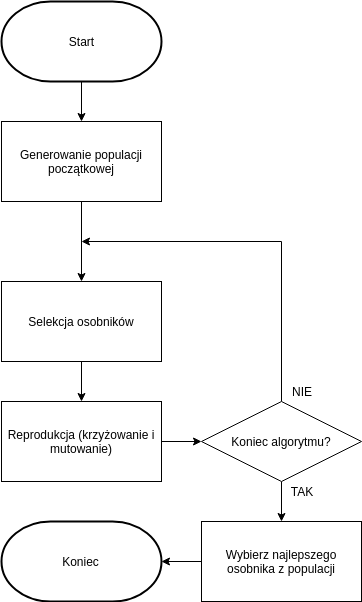
\includegraphics[width=6cm]{fig31.png}
	\caption{Schemat działania algorytmu genetycznego}
	\label{fig: 3.1}
\end{figure}

Proces selekcji polega na wytypowaniu najlepiej przystosowanych osobników za pomocą funkcji oceny oraz z niewielkim wpływem losowości. Krok ten realizowany jest na wiele różnych sposobów. Jednym z popularniejszych rozwiązań jest selekcja turniejowa. Polega ona na wytypowaniu losowych par osobników, które następnie poddane funkcji oceny określają osobnika lepszego i gorszego z danej pary. W tym wariancie do kolejnego kroku czyli reprodukcji przechodzą osobniki niekoniecznie najlepsze w stosunku do całej populacji. Inną implementacją tego etapu działania algorytmu jest metoda ruletki. Polega ona na losowaniu osobników przeznaczonych do dalszej reprodukcji z wirtualnego koła ruletki, w którym każdy osobnik ma swój wycinek tym większy im lepszy wynik osiągnął w funkcji oceny. Najprostszą metodą selekcji jest ranking polegający na posegregowaniu wszystkich kandydatów według ich oceny od najlepszego do najgorszego i udzielenie prawa do reprodukcji czołówce listy.

Po selekcji osobników następuje ich reprodukcja. Jest to proces polegający na mieszaniu struktury pozostałych kandydatów w celu uzupełnienia populacji po usunięciu wszystkich przegranych z poprzedniego kroku. W czasie działania procesu reprodukcji korzystamy z dwóch operatorów ewolucyjnych czyli krzyżowania i mutacji. Oba te operatory wykonują akcje na genotypie osobników, który jest zbiorem cech opisujących jednoznacznie danego osobnika (w tematykę genotypów i kodowania rozwiązań problemów zagłębię się bardziej w kolejnej sekcji tego rozdziału). Nazwy tych działań są łatwo zrozumiałe dla większości ludzi i bardzo dobrze opisują ich działanie. Pierwsza, czyli krzyżowanie, polega na pobraniu fragmentu cech jednego osobnika i uzupełnieniu ich cechami drugiego tak aby powstał kompletnie nowy osobnik będący losową mieszanką pierwszego i drugiego (Rysunek \ref{fig: 3.2}). 

\begin{figure}[h]
	\centering
	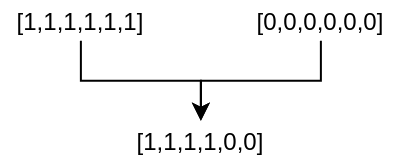
\includegraphics[width=6cm]{fig32.png}
	\caption{Przykład działania operacji krzyżowania genotypów dwóch osobników}
	\label{fig: 3.2}
\end{figure}

Następnie działamy operatorem mutacji na nowo powstałych kandydatach w celu wprowadzenia do populacji cech, które nie pojawiły się do tej pory. Odbywa się to z przyjętym wcześniej prawdopodobieństwem i polega na zmianie wartości pojedyńczej cechy zakodowanej w genotypie. Prawdopodobieństwo mutacji powinno być dość niskie. Zbyt wysoka ilość mutacji w populacji może prowadzić do zniszczenia dobrych wyników.

\section{Problem kodowania rozwiązania}

Samo działanie algorytmów genetycznych jest bardzo łatwe i przystępne do wytłumaczenia. Problem w implementacji takich tych technik znajduję w zupełnie innym miejscu a mianowicie w reprezentacji rozwiązań zadanego problemu w sposób umożliwiający przeprowadzanie na nich operacji zdefiniowanych przez teorię algorytmów genetycznych. Żeby dobrze zobrazować w czym tkwi problem musimy zdefiniować czym jest osobnik oraz genotyp w kontekście tej rodziny technik ewolucyjnych. Osobnikiem nazywamy tak na prawdę program komputerowy rozwiązujący przedstawiony problem lub jego konkretne rozwiązanie. Genotypem zaś nazywamy zbiór cech jednoznacznie opisujący danego osobnika. 

W odniesieniu do osobników jako programów ich genotyp zapisuje się w formie drzew syntaktycznych zamiast kodu \citep{poli08:fieldguide}. Natomiast w przypadku gdy nasi kandydaci reprezentują gotowe rozwiązania genotyp może być przedstawiany w formie wektora wartości definiujących rozwiązanie bądź również jako strukturę drzewiastą zależnie od potrzeb. Genotyp może się składać z jednego chromosomu i wtedy te pojęcia są tożsame jednak w przypadku dość rozbudowanych zagadnień stosuje się genotypy wielochromosomowe i składają się one wtedy z wielu drzew bądź wektorów cech poddawanych operacjom ewolucyjnym niezależnie od siebie.

Kodowanie osobników składających się na populację algorytmu jest bardzo ważnym i ciężkim zadaniem. Źle dobrana struktura genotypu może utrudnić a nawet uniemożliwić algorytmowi dotarcie na przestrzeni rozwiązań do punktów optymalnych tym samym ograniczając jego efektywność.

\section{Zastosowania}

Algorytmy genetyczne dzięki swojej elastyczności co  to dziedziny przestrzeni przeszukiwanej znajdują swoje zastosowanie w wielu obszarach nauki i przemysłu. Najbardziej podstawowym przykładem jest rozwiązywanie problemu komiwojażera, który przekłada się na zastosowanie ich na przykład w ustalaniu optymalnych tras dla logistyki towarów i zaopatrzenia. W takim wariancie pozwalają również na generowanie bardziej optymalnych architektur układów scalonych.

W swim artykule Panowie Grzegorz Chodak i Witold Kwaśnicki prezentują metody modelowania algorytmu genetycznego w celu prognozowania popytu. Takie zastosowanie jest według nich kolejnym etapem rozwoju metod prognozowania \citep{chodak2002zastosowanie}. W tym wypadku algorytm genetyczny potrafi dostarczyć informacje, które pozwalają na bardziej optymalne zarządzanie łańcuchem dostaw w firmach zajmujących się obrotem dobrami o sezonowym popycie ciężkim do przewidzenia dla ludzi. Z badań tych wynika, że algorytmy genetyczne znajdują wiele zastosowań w tradycyjnym biznesie i mogą pomagać przedsiębiorstwom w przewidywaniu wielu korzystnych i niekorzystnych zdarzeń na rynku co pozwala na dostosowanie strategii firm do tych warunków.

Jednej ze swoich prac profesor Zbigniew Michalewicz przeprowadzał badania zastosowania algorytmów ewolucyjnych, w tym algorytmów genetycznych, w problemie projektowania konstrukcji kratownicowej \citep{michalewicz1996evolutionary}. Z jej treści można wywnioskować, że ta rodzina algorytmów także może być przydatnym narzędziem w branży budowlanej i konstrukcyjnej. Jej zastosowanie pozwala na szybkie projektowanie optymalnych struktur, których człowiek mógłby nie zaprojektować.  

%%%%%%%%%%%%%%%%%%%%%%%%%%%%%%%%%%%%%%%%%%%%%%%%%%%%%%%%%%%%%%%%%%%%%%%%%%%%%%%%%%%%%

\chapter{Samouczący się bot do gry zręcznościowej}

Po przedstawieniu we wstępie tezy oraz przybliżeniu tematów z nią związanych chciałbym dogłębnie przedstawić zaprojektowany przez mnie sposób na jej sprawdzenie. w tym rozdziale po kolei przejdę po strukturze aplikacji napisanej na potrzeby przeprowadzenia doświadczeń związanych z tematem owej pracy. Przedstawię dokładny stoch technologiczny użyty do napisania tego kodu. w tym opisie uwzględnię krótkie opisy użytych bibliotek zewnętrznych. Zdefiniuję ideę działanie tego projektu oraz dokładnie zobrazuję strukturę kodu. Później dogłębnie przeanalizuję wyniki działania tego programu i przedstawię je w przystępnej i czytelnej formie.

\section{Stos technologiczny}

W ostatnich latach w branży informatycznej można zaobserwować ogromny wzrost popularności języka programowania Python. Według danych z największej na świecie ankiety przeprowadzanej wśród hobbistów i profesjonalnych programistów sporządzanej przez portal Stack Overflow (\textit{ang. Stack Overflow Annual Developer Survey}) \citep{stackoverflow-survey} język ten przeskoczył z 10 miejsca najbardziej lubianych języków programistów w 2015 roku na drugą pozycję pod koniec roku 2018. Jest to rozwijany jako projekt otwartoźródłowy język wysokiego poziomu ogólnego przeznaczenia. Cechuje się bardzo zwięzłą i przejrzystą składnią oraz działa na wielu systemach operacyjnych takich jak Windows, Linux czy MacOs. To właśnie dzięki swojej syntaktyce podobnej w pewnym stopniu do tej z pakietu MatLab oraz niskiemu progowi wejścia zyskał duże uznanie w kręgach naukowych jako narzędzie do łatwego zapisywania algorytmów i przeprowadzania skomplikowanych obliczeń matematycznych. Jego popularność w tych kręgach przeniosła się na powstanie dla niego wielu bibliotek zewnętrznych około naukowych w tym takie pakiety jak \textit{scikit-learn} czy \textit{tensorflow}. Z tych właśnie powodów mój wybór języka, w którym przetestuję postawioną tezę padł na Python'a.

Kolejną rzeczą wartą uwagi jest już wcześniej wspomniany pakiet \textit{tensorflow}. Jak możemy przeczytać na stronie głównej projektu jest to kompleksowa platforma open source do uczenia maszynowego. Posiada wszechstronny, elastyczny ekosystem narzędzi, bibliotek i zasobów tworzonych przez społeczność, który pozwala badaczom na wykorzystanie najnowocześniejszych rozwiązań nauczania maszynowego \citep{tensorflow-wesite}. Produkt ten tak zamo jak język Python jest kompletnie darmowy i udostępniony na licencji Apache 2.0. W moim projekcie posłuży on jako podstawowy silnik obliczeń dla tworzonych sieci neuronowych.

Przedstawiona powyżej biblioteka dostarcza ogromną liczbę narzędzi służących do kreowania rozwiązań z wykorzystaniem koncepcji sieci neuronowych i nauczania maszynowego. Jednakże za taką ilością możliwości jakie dostarcza użytkownikowi idzie skomplikowanie i trudność w szybkim programowaniu z jej użyciem. Ten problem rozwiązuje kolejne rozwiązanie zwane \textit{keras}. Pakiet ten jest wysokopoziomowym interfejsem programowania aplikacji (ang. \textit{application programming interface}) dla sieci neuronowych. Udostępnia on zestaw funkcji odpowiadający semantycznie teorii na temat sieci neuronowych pozwalający na szybkie i łatwe ich tworzenie i operowanie nimi osobą z wiedzą w tym temacie. Jednocześnie eliminuje potrzebę optymalizowania swojego kodu i wgłębiania się w sposób działania wybranego silnika nauczania maszynowego działającego pod spodem.

Ostatnim elementem stosu technologicznego projektu badającego tezę tej pracy jest \textit{pygame}. Jest to niewielka, otwartoźródłowa i darmowa biblioteka języka Python służąca do tworzenia aplikacji multimedialnych. Rozwija ją niewielka grupka hobbystów ale mimo tego zyskała swoją popularność dzięki dobrej wydajności i łatwości obsługi. Posłuży mi ona do stworzenia niewielkiej gry w węża (ang. \textit{snake}), która będzie odgrywać rolę funkcji oceny dla algorytmu genetycznego.

Reasumując cały głównymi filarami projektu jest język programowania Python i trzy bardzo popularne biblioteki dla niego stworzone czyli \textit{tensorflow}, \textit{keras} oraz \textit{pygame}. Zostały one przeze mnie wybrane nie tylko ze względu na wspomniane wcześniej zalety ale również z powodu ogromnej społeczności działającej w okół nich i zapewniającej ogromną ilość materiałów pomocniczych, które odgrywają wielką role w procesie uczenia się tych technologii.

\section{Reprezentacja sieci neuronowej w formie genotypu osobników algorytmu genetycznego}

Teraz po krótce chciałbym zdefiniować teoretyczną podstawę działania aplikacji bez wchodzenia w techniczne detale jej implementacji. Jest to ogólna idea, która przyświecała mi podczas przyglądania się technikom związanym ze współczesnymi algorytmami sztucznej inteligencji.

Na podstawie analizy przedstawionych przez mnie informacji na temat sztucznych sieci neuronowych oraz algorytmów genetycznych można dojść do kilku ciekawych wniosków. Jednym z nich jest to, że sieci neuronowe swój program działania powstały pod wpływem procesu uczenia w całości definiują za pomocą zestawu wag i przesunięć połączeń neuronowych. Wynika z tego, że modyfikowanie działania sieci odbywa się wyłącznie poprzez modyfikację wartości zawartych w takim zestawie. Teraz wracając na chwilę do algorytmów genetycznych możemy zauważyć, że poszukiwanie rozwiązania jest w nich realizowane za pomocą modyfikacji genów (cech) w genotypie, który jest zestawem genów. Analogia tych dwóch procesów naprowadza na wniosek o możliwości połączenia obydwu metod. Sieci neuronowe w swojej budowie i sposobie działania wpisują się w schemat reprezentacji osobnika po stronie algorytmu genetycznego.

Na tej teorii można zacząć konstruować algorytm genetyczny obierający sobie jako kandydatów rozwiązań wiele losowo wygenerowanych wariantów sztucznej sieci neuronowej o wcześniej określonej budowie topografii sieci. Przyglądając się wynikom jakie otrzymujemy za pomocą algorytmów genetycznych można spekulować, że taka symbioza technik sztucznej inteligencji ma możliwości doprowadzić do rezultatów lepszych pod względem ich jakości i wydajności.

\section{Opis działania i struktura projektu}

Cały projekt podzielony jest na dwa pakiety. Pierwszym z nich jest samodzielna gra w węża napisana za pomocą biblioteki \textit{pygame}. Uruchomienie gry jest w pełni konfigurowalne i pozwala na wybranie rozmiaru planszy, typu rozgrywki (gracz czy sieć neuronowa) oraz tępa gry. Zasady gry są dość proste. Poruszamy się po planszy o wybranych rozmiarach głową węża w czerech kierunkach: góra, dół, prawo, lewo. W każdym momencie gy zabronione jest poruszanie się do tyłu, czyli jeśli wąż porusza się do góry w danym momencie to w następnym ruchu nie może zacząć się przemieszczać w dół. Celem gracza jest zebranie jak największej ilości owoców, które pojawiają się na planszy w losowych miejscach. Zjedzenie owocu skutkuje zwiększeniem licznika punktów o 1 oraz wzrostem ogona węża, który podąża za graczem. Koniec gry następuje w chwili śmierci postaci wywołanej kontaktem z ogonem bądź wyjściem poza planszę gry. Aby zabezpieczyć się przed bieganiem po planszy w nieskończoność po jednej trasie w grze występuje limit kroków możliwych do wykonania od zjedzenia owocu. Wynikiem końcowym jest ilość zdobytych punktów oraz długość rozgrywki.

Dwa tryby różnią się od siebie tylko sposobem przyjmowania rozkazów przez grę. W trybie dla gracza polecenia wydawane są poprzez wciśnięcia klawiszy na klawiaturze komputera. Jeśli jednak podczas procesu uruchamiania zostanie przekazana sieć neuronowa to sygnały wejściowe z klawiatury zostają odcięte a polecenia są wykonywane na podstawie wartości wyjściowych sieci.

Drugim pakietem wchodzącym w skład projektu stworzonego na potrzeby przeprowadzenia badań do tej pracy jest moja własna implementacja algorytmu genetycznego. Podstawowym elementem tego algorytmu jest klasa kandydata rozwiązania, która przechowuje informacje na temat genotypu rozwiązania, którym w tym wypadku jest zestaw wag sieci neuronowej, oraz implementacje metod operatorów genetycznych takich jak krzyżowanie osobników i mutowanie genotypu. Klasa ta jest także odpowiedzialna za uruchamianie gry z użyciem jej genotypu oraz przechowywanie wyniku rozgrywki.

Działanie algorytmu odbywa się według schematu już opisanego przeze mnie w rozdziale drugim. Na początku generowana jest populacja początkowa obiektów wspomnianej wyżej klasy kandydata. Następnie w pętli uruchamiają się poszczególne fazy działania czyli selekcja, krzyżowanie i mutacja.

Selekcja osobników odbywa się trybem turniejowym. Kandydaci rozwiązań dobierani są w losowe pary a następnie każdy z nich uruchamia grę ze wstrzykniętą swoją siecią neuronową. Jeśli osobnik populacji żyje już kilka pokoleń to w każdym z nich przystępuje do rozgrywki a jako jego wynik obiera się najlepszy jaki udało mu się osiągnąć. Po wytypowaniu zwycięzców z par wszyscy przegrani zostają odrzuceni a reszta przechodzi do następnego etapu.

W fazie krzyżowania następuje wygenerowanie ruletki żyjących osobników na podstawie ich wyników. Im wyższy wynik tym większą część koła ruletki zajmuje dany kandydat. Teraz w pętli losowana jest para to krzyżowania aż liczba nowo otrzymanych rozwiązań będzie równa liczbie odrzuconych w poprzednim kroku algorytmu.

Ostatnim etapem jest przeprowadzenie losowych mutacji genotypów nowych rozwiązań. Algorytm dostaje wraz z konfiguracją ile mutacji ma przeprowadzić dla każdego pokolenia, gdzie jedna mutacja to zmiana tylko jednego pojedyńczego genu a w tym przypadku wagi jednego połączenia neuronowego danej sieci.

\section{Wyniki}

W tej sekcji opiszę proces uruchamiania projektu oraz wyniki jakie otrzymałem z jego pomocą. Aby dopełnić obraz przedstawię też na jakiej konfiguracji sprzętowej miał okazję działać algorytm. Wraz z kolejnymi uruchomieniami dochodziłem też do różnych wniosków dotyczących kodowania sieci neuronowej jak i doboru jej parametrów co poskutkowało dwoma różnymi podejściami dającymi bardzo odmienne wyniki.

\subsection{Platforma testowa i sposób pozyskania wyników}

Eksperymenty za pomocą napisanego projektu przeprowadzałem na moim prywatnym komputerze stacjonarnym klasy PC z zainstalowanym systemem operacyjnym Manjaro Linux. Sercem tej jednostki jest ośmiordzeniowy i szesnastowątkowy procesor firmy AMD z serii Ryzen 5 model 1400. W jego pracy wspomaga go 16GB pamięci ram oraz karta graficzna firmy Nvidia model GeForce GTX 960.

Podczas przeprowadzania obliczeń obciążenie wszystkich wątków procesora nie przekraczało 20-30 procent. Proces główny interpretera Python, który uruchamiał projekt zajmował przez cały czas działania nie więcej niż 300MB pamięci ram.

Do pozyskiwania wyników algorytm został wyposażony w moduł służący do zapisywania wielu statystyk do plików na dysku. Po zakończeniu obliczeń wszystkie dane można odczytać z 3 plików, które posiadają informacje o użytej konfiguracji i przebiegu algorytmu. Ostatni z tych plików to plik z rozszerzeniem .h5, w którym zapisana zostaje najlepsza sieć wygenerowana przez algorytm.

\subsection{Podejście pierwsze: obraz planszy jako dane wejściowe}

W pierwszym podejściu zacząłem od, jak mi się wydawało, najłatwiejszej implementacji, w której jako dane wejściowe do sieci neuronowej przekazywałem obraz z całej planszy. Generowana tablica dwuwymiarowa zawierała informacje o tym jaki obiekt znajduje się w danym momencie na każdym polu obszaru gry. Jednocześnie podjąłem decyzję aby wagi połączeń neuronowych w generowanych sieciach były liczbami rzeczywistymi z zakresu od -1 do 1. W tym wariancie mutacje genów odbywały się poprzez dodanie do wagi losowego współczynnika mutacji, który był losowany z zakresu -0.5 do 0.5. Sieci neuronowe w tym przykładzie składały się z warstwy wejściowej, warstwy wyjściowej z czterema neuronami i dwóch warstw ukrytych każda po 256 neuronów.

Wyniki pierwszego uruchomienia działającego według schematu podanego powyżej były wielce niezadowalające.
Algorytm pracował z 20 osobników na pokolenie przez 1000 pokoleń a wyniki przez niego otrzymane są zaprezentowane w na rysunku poniżej (Rysunek \ref{fig: 4.1}).

\begin{figure}[h]
	\centering
	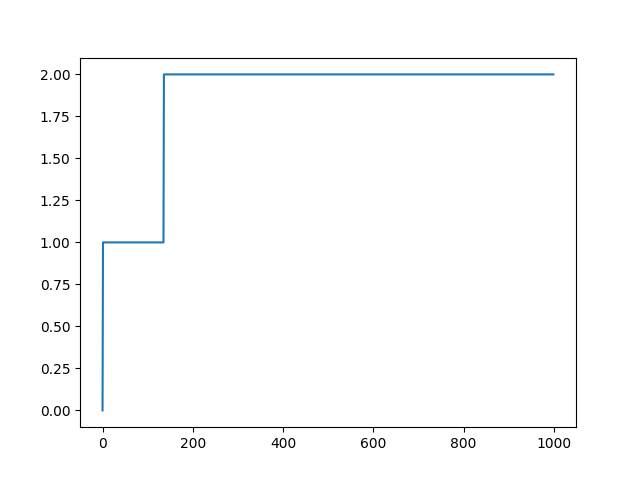
\includegraphics[width=8cm]{fig41.png}
	\caption{Wyniki uruchomienia pierwszego podejścia(20 osobników, 1000 pokoleń) }
	\label{fig: 4.1}
\end{figure}

Widoczne jest, że algorytm nie jest w stanie wygenerować odpowiedniej sieci mając do dyspozycji tylko 20 osobników na pokolenie. Następne uruchomienie postanowiłem skonfigurować na większą ilość osobników i pokoleń. Tym razem obliczenia były przeprowadzone dla 500 kandydatów przez 2000 iteracji i wyniki tego podejścia nie różniły się zbytnio od poprzednich (Rysunek \ref{fig: 4.2})

\begin{figure}[h]
	\centering
	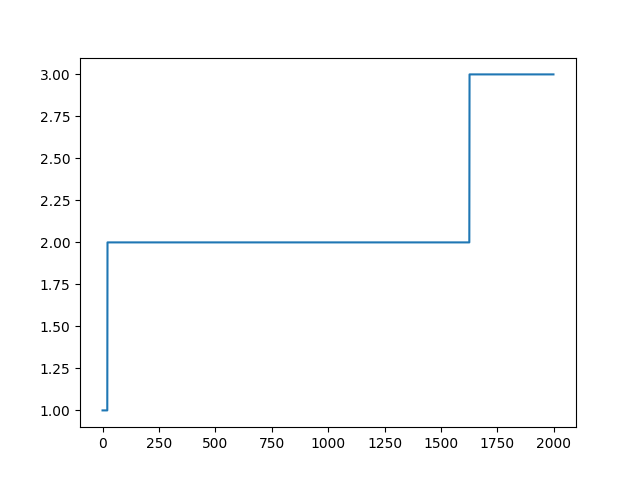
\includegraphics[width=8cm]{fig42.png}
	\caption{Wyniki uruchomienia pierwszego podejścia(500 osobników, 2000 pokoleń) }
	\label{fig: 4.2}
\end{figure}

Teraz ewidentnie widać, że to podejście jest bardzo nieoptymalne. Analizując działanie tak wygenerowanych sieci neuronowych można zauważyć, że jakiekolwiek zdobyte punkty w grze były tylko zbiegiem okoliczności a one nie rozpoznają prawie żadnych sytuacji na planszy. Ruchy w grze są kompletnie losowe i niezależne od tego co dzieje się podczas rozgrywki.

Sieci z tak zaprojektowanym wejściem musiałyby mieć zestaw wag połączeń neuronowych, które odzwierciedlałyby każda możliwą kombinację planszy gry. Przy takim podejściu potrzebowalibyśmy sieci neuronowych o ogromnej liczbie sztucznych neuronów co dodatkowo komplikuje i wydłuża obliczenia.

\subsection{Podejście drugie: widok z głowy węża jako dane wejściowe}

W drugim wariancie postanowiłem uprościć wiele aspektów sieci neuronowych generowanych za pomocą algorytmu. Pierwszym uproszczeniem była warstwa wejściowa sieci i dane, które są do niej przekazywane. zamiast tworzyć ogromną strukturę wejścia zależną od rozmiarów planszy, czyli też działającą tylko dla jednego wariantu gry, postanowiłem skonstruować wejście na podstawie tego co widzi w grze wąż ze swojej perspektywy. 

Taka struktura składa się z 24 sygnałów. Pierwsze osiem reprezentuje w jakim kierunku wąż widzi następny owoc, kolejne odpowiadają za widzenie ogona. Wszystkie pierwsze 16 sygnałów przyjmuje wartości albo 0 albo 1 i sygnalizuje jedynie obecność obiektu w danym kierunku. Ostatnie osiem sygnalizuje odległości od granic planszy, przyjmuje wartość ciągłą od 0 do 1, im mniejsza wartość sygnału tym dalej od ściany znajduje się wąż.

Kolejnym uproszczeniem była zmiana możliwych wartości wag. Teraz połączenia neuronowe tylko przesyłają sygnał niezmieniony albo zmieniają jego znak, czyli przyjmują wartości 1 albo -1. Mutowanie odbywa się teraz poprzez zmianę znaku wagi połączenia neuronowego.

Sama architektura sieci też się zmieniła i teraz obydwie warstwy ukryte składają się jedynie z dwudziestu neuronów. Dzięki temu złożoność obliczeniowa sieci drastycznie spadła pozwalając na dużo szybsze podejmowanie decyzji o kolejnym ruchu.

Z takimi zmianami przystąpiłem do ponownych uruchomień algorytmu aby zobaczyć wyniki. Pierwszą próbę przedstawiłem poniżej (Rysunek \ref{fig: 4.3}) i wygląda ona znacznie bardziej obiecująco.

\begin{figure}[h]
	\centering
	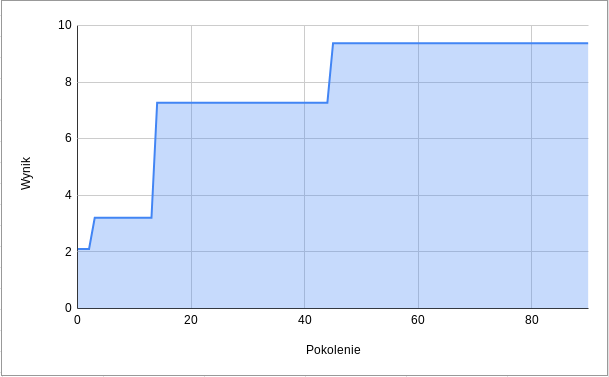
\includegraphics[width=8cm]{fig43.png}
	\caption{Wyniki uruchomienia drugiego podejścia(2000 osobników, 100 pokoleń) }
	\label{fig: 4.3}
\end{figure}

Uproszczenie struktury sieci neuronowej pozwoliło na analizowanie większej ilości rozwiązań w krótszym czasie. Jednocześnie sygnały wejściowe dużo lepiej opisują w tym wariancie warunki wpływające na podjęcie decyzji o kolejnym ruchu.
 
%%%%%%%%%%%%%%%%%%%%%%%%%%%%%%%%%%%%%%%%%%%%%%%%%%%%%%%%%%%%%%%%%%%%%%%%%%%%%%%%%%%%%

\chapter{Wnioski}

\pagebreak
%%%%%%%%%%%%%%%%%%%%%%%%%%%%%%%%%%%%%%%%%%%%%%%%%%%%%%%%%%%%%%%%%%%%%%%%%%%%%%%%%%%%%
\bibliographystyle{plainnat}
\addcontentsline{toc}{chapter}{Bibliografia}
\bibliography{bibliography}

\end{document}